\begin{center}
    \bfseries Interfacing Ultrasonic Sensor with Arduino - Python
\end{center}
\section{Ultrasonic Sensor:}
The HC-SR04 ultrasonic sensor uses SONAR (Sound Navigation and Ranging) to determine the distance of an object just like the bats do. It offers excellent non-contact range 
detection with high accuracy and stable readings in an easy-to-use package from 2 cm to 400 cm or 1” to 13 feet. The operation is not affected by sunlight or black material, although acoustically, soft materials like cloth can be difficult to detect. It comes complete with ultrasonic transmitter and receiver module.


\section{Technical Specifications:}
\begin{itemize}
\item Power Supply − +5V DC
\item Quiescent Current − <2mA
\item Working Current − 15mA
\item Effectual Angle − <15°
\item Ranging Distance − 2cm – 400 cm/1″ – 13ft
\item Resolution − 0.3 cm
\item Measuring Angle − 30 degree

\end{itemize}

\vspace{1cm}
\section{Interfacing Ultrasonic Senor With Arduino:}
\textbf{Components Required:}
\begin{itemize}
\item 1 × Arduino Uno R3
\item 1 × ULTRASONIC Sensor (HC-SR04)
\item 4 x Jumper Wires
\end{itemize}


\section{Circuit Diagram}

Here is a illustration of the circuit which has to make for this experiment. This is simulated using TINKERCAD , an online platform to simulate circuits.
\begin{figure}[ht]
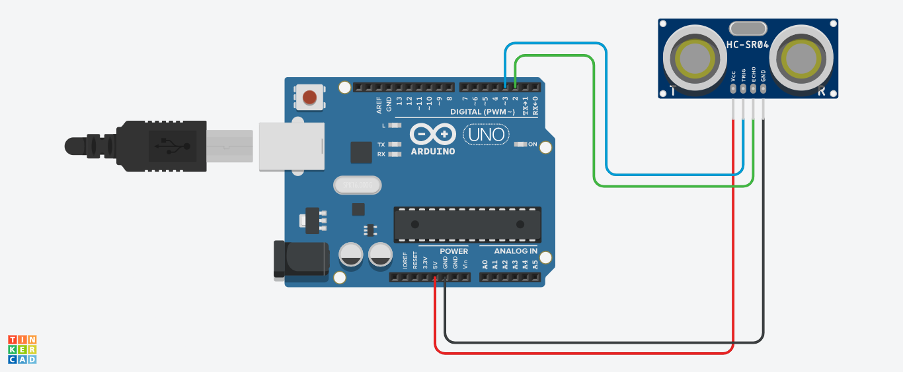
\includegraphics[width=13cm]{VITC/images/Picture 1.png}
\caption{Circuit Diagram}
\end{figure}


\section{Arduino Code:}
\lstset{language=Python}
\lstset{frame=lines}
\lstset{caption={Arduino Code}}
\lstset{label={lst:code_direct}}
\lstset{basicstyle=\footnotesize}
\begin{lstlisting}
#define echoPin 2
#define trigPin 3
long duration;
int distance;
void setup(){
Serial.begin(9600);
pinMode(trigPin,OUTPUT);
pinMode(echoPin,INPUT);
}
void loop(){
digitalWrite(trigPin,LOW);
delayMicroseconds(2);
digitalWrite(trigPin,HIGH);
delayMicroseconds(10);
digitalWrite(trigPin,LOW);

duration=pulseIn(echoPin,HIGH);
distance=(duration*0.034/2);
Serial.print("Distance : ");
Serial.print(distance);
Serial.println(" cm ");
delay(1000);
}

\end{lstlisting}



\\
\section{Code Explanation:}
\textbf{Step 1:}
    Open the Arduino IDE and we need define two pins, echoPin on digital pin 2 and trigPin on digital pin 3. by using the keyword "define'. Next declare two variables, one is "duration". This is for store the duration of sound wave travelled. Other is "distance" for store the distance calculated.\\
\lstset{language=Python}
\lstset{frame=lines}

\lstset{label={lst:code_direct}}
\lstset{basicstyle=\footnotesize}
\begin{lstlisting}
#define echoPin 2
	#define trigPin 3
	long duration;
	int distance;
\end{lstlisting}


\textbf{Step 2:}
    In the void setup() function we need to begin the serial communication with baurd rate as 9600. It is done by the keyword "Serial.begin(9600)". Then set the trigPin as "OUTPUT", by the keyword "pinMode(trigPin, OUTPUT)". Because the trigPin is the input pin of transmitter of sensor module. Now we need to set the echoPin as "INPUT". By the keyword "pinMode(echoPin, INPUT)".\\
\lstset{language=Python}
\lstset{frame=lines}

\lstset{label={lst:code_direct}}
\lstset{basicstyle=\footnotesize}
\begin{lstlisting}
void setup(){
  			Serial.begin(9600);
 			pinMode(trigPin,OUTPUT);
  			pinMode(echoPin,INPUT);
 		}
\end{lstlisting}

\textbf{Step 3:}
    Now the trigPin state is in a float condition. We need to set it as "LOW". for this purpose we use the keyword "digitalWrite(trigPin, LOW)". Then hold this state for 2 microseconds by the keyword "delayMicroseconds(2)".\\
\lstset{language=Python}
\lstset{frame=lines}

\lstset{label={lst:code_direct}}
\lstset{basicstyle=\footnotesize}
\begin{lstlisting}
    digitalWrite(trigPin,LOW);
	delayMicroseconds(2);

\end{lstlisting}

    Now we need to set the trigPin "HIGH" for 10 seconds, with the same keyword mentioned above. Only change the parameter.Then set the trigPin as "LOW" state.
\lstset{language=Python}
\lstset{frame=lines}

\lstset{label={lst:code_direct}}
\lstset{basicstyle=\footnotesize}
\begin{lstlisting}
digitalWrite(trigpin,HIGH);
delayMicroseconds(10);

digitalWrite(trigpin,LOW);

\end{lstlisting}
Now read the echoPin and put it to the function "pulseIn(echoPin, HIGH)". This returns the total travel time. So we need to store this return value to the variable "duration".\\

\lstset{language=Python}
\lstset{frame=lines}
\lstset{label={lst:code_direct}}
\lstset{basicstyle=\footnotesize}
\begin{lstlisting}
duration=pulseIn(echoPin,HIGH);
\end{lstlisting}
    The total travel time is now stored in the variable "duration"
    Now we can calculate the distance from this duration by using the equation. And store calculated value(distance) to the variable "distance". The equation is explained above\\
\begin{center}
    \textbf{distance=(duration*0.034/2);}
\end{center}\\
The distance from the sensor to the object is now stored in the variable "distance".
Then we need to display it to screen. For this purpose, here we using the serial communication. You can also use LCD, Sven Segment Display, OLED Display, etc...(The will change). First print a headingor a message. Here I am going to print "Distance". by using "Serial.print("Distance : " )". After that print the distance to the serial monitor, we use the keyword "Serial.println(distance)". Then print the unit by "Serial.println(" cm ")". Here I used a "ln" with "Serial.print()". It's for start a new line. The code is like,then add Delay.
\lstset{language=Python}
\lstset{frame=lines}
\lstset{label={lst:code_direct}}
\lstset{basicstyle=\footnotesize}
\begin{lstlisting}
    Serial.print("Distance : " );
    Serial.print(distance)";
    Serial.println(" cm ")";
	
	delay(1000);

\end{lstlisting}
\vspace{10pt}
\section{Python Code:}
\lstset{language=Python}
\lstset{frame=lines}
\lstset{caption={Python Code}}
\lstset{label={lst:code_direct}}
\lstset{basicstyle=\footnotesize}
\begin{lstlisting}
import os 
import sys
import time

cwd = os.getcwd()
(setpath,Examples) = os.path.split(cwd)
sys.path.append(setpath)

from Arduino import Arduino
from time import sleep

class HCSR04:
    def __init__(self, baudrate):
        self.baudrate = baudrate
        self.setup()
        self.run()
        self.exit()

    def setup(self):
        self.obj_arduino = Arduino()
        self.port = self.obj_arduino.locateport()
        self.obj_arduino.open_serial(1, self.port, self.baudrate)

    def run(self):
        self.echo = 8
        self.trig = 9
        while True:
            st=self.obj_arduino.cmd_dist(1,self.trig,self.echo)
            print(st)
            sleep(1)
            
    def exit(self):
        self.obj_arduino.close_serial()

def main():
    obj_hcsr04 = HCSR04(115200)

if __name__=='__main__':
    main()

\end{lstlisting}


